% Standalone technical-supplement body. Compile through TechnicalSupplement.tex.
% This file is intentionally not input by the submitted main paper.

\appendix

\section{Scope and Artifact Organization}
This supplement expands the reproducibility and diagnostic evidence for the
submitted paper. It does not introduce a new task, metric, model, or claim. The
main paper remains self-contained; the material below gives exact
configurations, data provenance, controller details, and extended results that
are useful for auditing or reproducing the reported experiments.

The accompanying code-and-data archive contains the method-specific source for
dual-loop allocation, the exact 500-scenario training manifest, a launch
configuration, controller regression tests, manifest validation, and the
per-scenario SAGE outputs for the three complete-method runs. It does not contain
API credentials, proprietary model weights, a generic RL framework, or
third-party benchmark packages.
All paths in this document are relative to the root of that archive.

\begin{table}[t]
\centering
\small
\begin{tabular}{p{0.34\columnwidth}p{0.56\columnwidth}}
\toprule
Archive path & Contents \\
\midrule
\path{data/train_scenarios.jsonl} & Exact 500-scenario training manifest \\
\texttt{method/} & Controller, state construction, and rollout integration \\
\texttt{launch/} & Reproduction launch configuration \\
\texttt{tests/} & Controller and interaction-state regression tests \\
\texttt{scripts/} & Validation and SAGE-summary utilities \\
\texttt{results/sage/} & Three per-scenario SAGE outputs and run summary \\
\bottomrule
\end{tabular}
\caption{Organization of the anonymous code-and-data archive.}
\label{tab:supp-artifact-layout}
\end{table}

\section{Data Provenance and Evaluation Isolation}
\subsection{Training Scenario Provenance}
The 500 training scenarios are inherited from the public RLVER release cited
in the main paper; they are not introduced as a new dataset by this work. The
file bundled at \texttt{data/train\_scenarios.jsonl} is the deterministic prefix
of length 500 from the upstream \texttt{data/train\_profile.jsonl} release. We
preserve the original record order and the fields used by training: a unique
identifier, persona, complete event description, behavioral tendencies, and
hidden support intent. No test scenario is appended to this file.

\begin{table}[t]
\centering
\small
\begin{tabular}{ll}
\toprule
Property & Value \\
\midrule
Archive path & \texttt{data/train\_scenarios.jsonl} \\
Source & Public RLVER training profiles \\
Selection rule & First 500 records, original order \\
Number of records & 500 \\
Unique support intents & 8 \\
SHA-256 & \texttt{82e09e73...fa53a3} \\
\bottomrule
\end{tabular}
\caption{Provenance of the exact training manifest.}
\label{tab:supp-data-provenance}
\end{table}

The complete SHA-256 checksum is
\texttt{82e09e73a89bf6e167fe8e56823aaa5e}\linebreak
\texttt{62b0bd55c1d08ef9618011aeb7fa53a3}.

The source release remains the authority for its terms of use. We include the
exact manifest in the anonymous archive so that the scenario population and
ordering used in the experiments can be verified without reconstructing the
subset. The archive records the upstream paper, source file, deterministic
selection rule, record count, and checksum.

\subsection{Splits and Isolation}
The 500 training scenarios, the development split used for configuration and
checkpoint selection, and the 100-scenario SAGE test set are instance-disjoint.
Test instances are never loaded by the training launcher, never update the
controller, and never participate in model selection. The launcher validates
that the training JSONL has exactly 500 records, unique identifiers, all
required fields, and eight non-empty support-intent categories before starting
distributed workers.

EIBench uses its fixed held-out test split of 213 scenarios: 51 Support, 64
Defense, 52 Repair, and 46 Charm. This split is used only for final evaluation.
ESC-Eval uses 331 fixed-role interactions under its official evaluation
protocol, and ESConv uses 2,895 reference responses. These evaluation resources
are kept outside the training archive and are not accessed by the controller.

\subsection{Independent Evaluation Surfaces}
Training simulation and emotion verification use DeepSeek-V3. Transfer is
measured through independent surfaces: the official InternLM2 plus ESC-RANK
pipeline for ESC-Eval, Qwen3-Max for EIBench, reference-based metrics for
ESConv, and blinded human ratings. Thus, the cross-benchmark results do not
reuse the training verifier. The SAGE result measures the target interactive
capability, whereas ESC-Eval, EIBench, ESConv, and human ratings test whether
the learned behavior transfers beyond that training-facing signal.

\section{Information Flow and Prompt Visibility}
For each rollout environment, the user simulator receives the complete scenario
and one hidden interaction state. The state is rendered as natural-language
behavioral guidance that regulates disclosure, emotional activation, and
relational trust while requiring preservation of the original persona, event,
and support need. The assistant receives only the alternating natural-language
dialogue. It never receives the support-intent label, state identifier, state
levels, controller statistics, sampling probabilities, pass rate, or a
difficulty label.

After the dialogue ends, the verifier scores the complete trajectory. The
continuous score is passed to GRPO as the policy reward. The controller receives
the same scores together with simulator-side intent and state identifiers, then
stores only group-level sufficient statistics. This separation is summarized
below.

\begin{table*}[t]
\centering
\small
\begin{tabular}{lp{0.24\textwidth}p{0.28\textwidth}p{0.25\textwidth}}
\toprule
Component & Observes & Produces & Does not observe \\
\midrule
Assistant policy & Dialogue text & Assistant turns & Intent/state labels, controller values \\
User simulator & Scenario, hidden state, dialogue history & User turns & Controller statistics \\
Emotion verifier & Complete trajectory & Continuous emotion outcome & Sampling probabilities \\
Controller & Intent/state IDs, completed-group outcomes & Next state distribution & Policy tokens or gradients \\
\bottomrule
\end{tabular}
\caption{Information available to each component. Simulator-side metadata is
not exposed to the assistant policy.}
\label{tab:supp-information-flow}
\end{table*}

\section{Exact Interaction-State Construction}
\subsection{State Axes}
The interaction space is the Cartesian product of three operational axes. They
describe how a user participates in a support dialogue rather than assigning a
clinical trait or changing the underlying event.

\begin{itemize}
  \item \textbf{Disclosure readiness} has three levels: delayed, conditional,
  and proactive. It controls the pace at which relevant details and deeper
  needs become available.
  \item \textbf{Emotional activation} has two bounded levels: moderate and
  high. It controls the intensity of negative-affect expression while
  preserving coherent role-play and safety constraints.
  \item \textbf{Relational trust} has four levels, from strong skepticism to
  sustained engagement. It controls whether the user accepts questions,
  validation, and proposed support.
\end{itemize}

Their product gives $3\times2\times4=24$ states. If
$z=(d,a,r)$, the simulator-side instruction is composed deterministically as
$\phi(z)=\phi_d(d)\oplus\phi_a(a)\oplus\phi_r(r)$. The exact UTF-8 strings are
defined in the released prompt-construction source; the English descriptions
below specify their behavior.

\subsection{Behavioral Clauses}
\paragraph{Disclosure, delayed.}
Reveal few details at a time and disclose deeper feelings only after the
assistant demonstrates sustained understanding.
\paragraph{Disclosure, conditional.}
Explain the basic difficulty and answer questions, while withholding sensitive
details until responses are specific, respectful, and affectively relevant.
\paragraph{Disclosure, proactive.}
Proactively describe events, feelings, and key context while preserving a
natural conversational pace.
\paragraph{Activation, moderate.}
Express clear but controlled negative affect with coherent language and without
repeated catastrophic wording.
\paragraph{Activation, high.}
Express strong negative affect, potentially including self-blame, anxiety,
anger, or catastrophic interpretation, without inventing an unsupported crisis.
\paragraph{Trust, level 1.}
Question whether the assistant truly understands, reject generic reassurance,
and withhold acceptance until responses are concrete and situated.
\paragraph{Trust, level 2.}
Continue cautiously, observe whether the assistant listens, and avoid
immediately accepting comfort or advice.
\paragraph{Trust, level 3.}
Accept reasonable empathy while remaining reserved toward empty, didactic, or
off-topic responses.
\paragraph{Trust, level 4.}
Presume good intent, engage with situation-specific support, and become more
receptive after feeling understood.

Every composed instruction ends with invariants: realize the condition only
through dialogue behavior; preserve the original persona, event facts, and
hidden support need; and never reveal dimension names, levels, state IDs,
difficulty labels, or system metadata. No random auxiliary goal or fourth state
dimension is appended.

\subsection{Support-Intent Factorization}
The complete scenarios retain their native hidden support intents. The
controller groups them into eight intent categories and maintains statistics
for each intent--state unit, giving $8\times24=192$ reusable units. Individual
scenario identities remain available to the simulator; factorization changes
only the level at which evidence is shared.

\begin{table}[t]
\centering
\small
\begin{tabular}{lr}
\toprule
Support intent & Training scenarios \\
\midrule
Validation of no fault & 66 \\
Guided self-reflection & 66 \\
Dialectical event analysis & 66 \\
Deep emotional empathy & 64 \\
Attentive emotional listening & 63 \\
Perspective taking about others & 60 \\
Actionable advice & 58 \\
Specific sincere praise & 57 \\
\midrule
Total & 500 \\
\bottomrule
\end{tabular}
\caption{Native support-intent composition of the training manifest.}
\label{tab:supp-training-intents}
\end{table}

\section{Controller Implementation}
\subsection{Group-Shared Outcomes}
For a sampled scenario $x$ with native intent $c$ and selected state $z$, all
$K$ rollouts in one GRPO group share $(x,z)$. The verifier returns continuous
outcomes $R_1,\ldots,R_K$. The policy uses those continuous values, whereas the
controller computes $y_k=\mathbb I[R_k\geq\eta]$ and the group pass rate
$p_m=K^{-1}\sum_k y_k$ for unit $m=(c,z)$. One complete group contributes one
controller observation. Incomplete groups or groups containing a non-finite
reward do not change controller history.

\subsection{Hierarchical Evidence and Sampling}
For every unit $(c,z)$, the controller stores the number of completed groups
$N_{c,z}$ and cumulative group pass rate $S_{c,z}$. Sparse units borrow evidence
from the same state in the other seven intents through the leave-one-intent
estimate described in the main paper. This estimate is converted into a bounded
boundary score, combined with an uncertainty bonus, and mixed with a uniform
distribution. The uniform component guarantees a non-zero probability for
every state throughout training.

The controller first collects 1,600 completed groups under uniform sampling
over all 24 interaction states. With a scenario batch of 16, this corresponds to approximately 100
optimizer steps, subject to complete-group accounting. It then samples from the
feedback-guided distribution. Scenario sampling remains uniform throughout;
only the conditional state distribution for each support intent changes.

\subsection{Persistence and Resume Semantics}
All rollout workers share a transactional SQLite database. Each completed group
updates global, state-level, and intent--state statistics atomically. The
database uses write-ahead logging, a busy timeout, and retry logic for concurrent
startup. The launcher places it on a local POSIX filesystem because SQLite
locking is not reliable on object-store mounts. For an interrupted run, this
database is copied to durable storage and supplied on restart through
\texttt{EGSEC\_CONTROLLER\_STATE\_FILE}, alongside the resumed policy checkpoint.
This restores controller counts, pass-rate sums, and the initialization state. A
regression test verifies that an incomplete group leaves both global and unit
statistics unchanged.

\section{Training and Controller Configuration}
\begin{table*}[t]
\centering
\small
\begin{tabular}{llll}
\toprule
Category & Setting & Value & Notes \\
\midrule
Policy & Backbone & Qwen3-8B & Non-thinking mode \\
Policy & Optimizer & AdamW & $\beta_1=0.9$, $\beta_2=0.999$, weight decay 0.01 \\
Policy & Learning rate & $3\times10^{-7}$ & Constant schedule, 0.02 warm-up ratio \\
Policy & PPO epochs / clip ratio & 1 / 0.2 & Gradient clipping 10.0 \\
Policy & KL coefficients & 0.01 / 0.01 & KL controller / actor KL loss \\
Policy & KL estimator & \texttt{low\_var\_kl} & Shared by matched RL systems \\
Rollout & Scenario batch / group size & 16 / 4 & 64 trajectories per optimizer step \\
Rollout & Policy temperature / top-$p$ & 1.0 / 1.0 & vLLM rollout policy \\
Rollout & Maximum dialogue turns & 8 & Multi-turn simulator interaction \\
Rollout & Prompt / response limits & 25,000 / 6,000 & Tokens \\
Rollout & Per-turn / PPO token limits & 6,000 / 32,000 & Tokens \\
Training & Optimizer steps & 500 & Checkpoints saved every 5 steps \\
Controller & Uniform collection & 1,600 groups & Completed groups, not trajectories \\
Controller & Success criterion $\eta$ & 50 & Controller only \\
Controller & Shrinkage $\lambda$ / prior $\alpha$ & 4 / 4 & Hierarchical pass-rate estimate \\
Controller & Uncertainty weight $\beta$ & 0.15 & UCB-style revisit bonus \\
Controller & Uniform mixture $\epsilon$ & 0.10 & Persistent rehearsal \\
Controller & Sampling temperature $\gamma$ & 1.0 & Applied to state scores \\
Controller & Minimum score $A_{\min}$ & 0.05 & Positive allocation floor \\
Simulator & Model / API temperature & DeepSeek-V3 / 0.7 & Frozen user and emotion scorer \\
Seeds & Scenario / profile pool & 2026 / 20260701 & Worker rank offsets scenario RNG \\
\bottomrule
\end{tabular}
\caption{Final training and controller configuration for the principal
Qwen3-8B experiments.}
\label{tab:supp-training-config}
\end{table*}

All controlled RL systems use the same policy initialization, simulator,
verifier, rollout budget, group size, context limits, optimizer settings, and
hardware. The policy reward consumed by GRPO is the continuous terminal emotion
outcome. Thresholding is used only by the outer-loop controller.

Training uses four NVIDIA A800 80GB GPUs on one GU108 instance. The released
environment snapshot records PyTorch 2.5.1 with CUDA 12.4 support,
Transformers 4.48.3, Ray 2.42.1, and the corresponding vLLM development build.

\section{Evaluation Protocol Details}
\subsection{Automatic and Interactive Evaluation}
SAGE evaluates 100 multi-turn scenarios and reports mean final emotion together
with success and failure rates under the official high- and low-emotion
criteria. ESC-Eval evaluates 331 fixed-role interactions with the official
InternLM2 and ESC-RANK pipeline on a 0--4 scale. EIBench uses 213 held-out
scenarios and reports its aggregate raw reward. ESConv uses 2,895 reference
responses and reports strategy accuracy, BLEU-2, ROUGE-L, BERTScore, and
Distinct-2; the paper multiplies these metrics by 100.

RLVER and the complete framework are trained independently three times. The
remaining fixed-checkpoint systems are evaluated three times under shared
evaluation seeds. Sample standard deviations are reported for aggregate
automatic metrics in the main table. The single-run component table compares
all ablations against the same complete-framework run, whose SAGE Overall is
78.11; the three-run complete-framework mean is 79.24.

\subsection{Human Evaluation}
Three annotators who are blind to system identity independently rate each
system dialogue for 100 randomly selected held-out scenarios. Dialogue order
and system order are randomized. The 0--4 overall-support rubric covers empathy,
contextual relevance, helpfulness, and dialogue coherence. Scores are first
averaged across the three annotators for each system--scenario pair and then
averaged across scenarios. Ordinal Krippendorff's $\alpha$ is 0.78.

\section{Extended SAGE Results}
\subsection{Independent Training Runs}
\begin{table}[t]
\centering
\small
\begin{tabular}{lrrrr}
\toprule
Method & Run 1 & Run 2 & Run 3 & Mean $\pm$ SD \\
\midrule
RLVER & 70.03 & 72.23 & 73.76 & $72.01\pm1.88$ \\
Ours & 81.02 & 78.58 & 78.11 & $\mathbf{79.24\pm1.56}$ \\
\bottomrule
\end{tabular}
\caption{SAGE Overall across three independent training runs. SD is the sample
standard deviation across runs.}
\label{tab:supp-independent-runs}
\end{table}

The weakest complete-framework run (78.11) exceeds the strongest RLVER run
(73.76). The gain therefore appears throughout the observed independent-run
range rather than being determined by one favorable optimization run.

\subsection{Outcome Distribution}
\begin{table}[t]
\centering
\small
\begin{tabular}{lrrrrr}
\toprule
Method & S & A & B & C & F \\
\midrule
Qwen3-8B & 20 & 25 & 15 & 11 & 29 \\
RLVER & 39 & 27 & 11 & 11 & 12 \\
Interaction State Only & 30 & 35 & 12 & 4 & 19 \\
Scenario-only allocation & 48 & 20 & 9 & 11 & 12 \\
\textbf{Ours} & \textbf{48} & \textbf{29} & \textbf{7} & \textbf{4} & \textbf{12} \\
\bottomrule
\end{tabular}
\caption{SAGE grade counts on one shared 100-scenario evaluation manifest.
Higher grades are better.}
\label{tab:supp-sage-grades}
\end{table}

Compared with RLVER, the complete framework moves nine additional scenarios
into grade S and two additional scenarios into grade A while reducing the
combined B/C mass. Scenario-only allocation reaches the same S count but leaves
more scenarios in C, showing why the full distribution is more informative
than success count alone.

\begin{table}[t]
\centering
\small
\setlength{\tabcolsep}{2pt}
\begin{tabular}{lrrrrr}
\toprule
Support intent & $n$ & Base & Uniform & Ours & $\Delta$\\
\midrule
Causal analysis      & 11 & 38.18 & 36.18 & \textbf{67.73} & $+31.55$\\
Emotional venting    & 12 & 61.92 & \textbf{85.92} & 84.17 & $-1.75$\\
Stance affirmation   & 11 & 61.82 & 91.36 & \textbf{99.09} & $+7.73$\\
Deep empathy         & 13 & 74.85 & 85.69 & \textbf{94.23} & $+8.54$\\
Dialectical analysis & 12 & 46.25 & 81.25 & \textbf{84.42} & $+3.17$\\
Actionable advice    & 15 & 43.67 & 55.27 & \textbf{57.67} & $+2.40$\\
Specific praise      & 13 & 78.46 & \textbf{80.77} & 79.62 & $-1.15$\\
Guided reflection    & 13 & 26.23 & 63.15 & \textbf{67.31} & $+4.15$\\
\bottomrule
\end{tabular}
\caption{SAGE emotion score by hidden support intent on one matched 100-scenario evaluation manifest. $\Delta$ compares the complete framework with uniform emotion-reward RL.}
\label{tab:intent-breakdown}
\end{table}


Table~\ref{tab:intent-breakdown} asks whether the aggregate gain is confined to
one hidden support need. The complete framework improves over RLVER in six of
eight intent categories. The largest margin occurs for causal analysis, where
the counselor must move beyond generic validation and help the user reason
about another person's behavior. Because individual categories contain only
11--15 test scenarios, this table is used as a diagnostic breakdown rather than
a separate significance claim.

\section{Extended Cross-Benchmark Results}
\subsection{ESC-Eval Dimensions}
\begin{table*}[t]
\centering
\small
\begin{tabular}{lcccccccc}
\toprule
Counselor training
& Flu. & Div. & Emp. & Sug. & Hum. & Tech. & Overall & Macro \\
\midrule
Qwen3-8B
& 2.78 & 2.55 & 2.46 & 2.31 & 1.72 & 2.64 & 2.27 & 2.39 \\
RLVER
& 2.86 & 2.68 & 2.61 & 2.43 & 1.82 & 2.73 & 2.30 & 2.49 \\
Interaction State Only
& 2.82 & 2.64 & 2.52 & 2.37 & 1.79 & 2.69 & 2.18 & 2.43 \\
\textbf{Ours}
& \textbf{2.91} & \textbf{2.74} & \textbf{2.72} & \textbf{2.52}
& \textbf{1.88} & \textbf{2.74} & \textbf{2.34} & \textbf{2.55} \\
\bottomrule
\end{tabular}
\caption{Detailed results under the official ESC-Eval protocol. All dimensions
use the original 0--4 scale; Macro is the arithmetic mean of the seven columns.}
\label{tab:supp-esc-dimensions}
\end{table*}

The complete framework improves every ESC-Eval dimension over Qwen3-8B and
RLVER. The largest margins over RLVER occur for empathy and suggestion quality,
while fluency, diversity, humanness, technical quality, and overall quality are
also maintained or improved.

\subsection{EIBench Categories}
\begin{table}[t]
\centering
\small
\setlength{\tabcolsep}{2pt}
\begin{tabular}{lrrrrr}
\toprule
Method & Overall & Support & Defense & Repair & Charm \\
\midrule
Qwen3-8B & -22.40 & -43.30 & -21.40 & -35.90 & 14.60 \\
RLVER & -9.79 & -34.27 & -2.55 & -14.72 & 12.80 \\
States Only & -40.60 & -75.17 & -12.66 & -51.52 & -28.83 \\
\textbf{Ours} & \textbf{-7.55} & \textbf{-27.61} & -6.31 & \textbf{-11.64} & \textbf{17.52} \\
\bottomrule
\end{tabular}
\caption{EIBench raw rewards by category under one shared 213-scenario
evaluation protocol. Higher is better.}
\label{tab:supp-eibench-categories}
\end{table}

The complete method obtains the highest aggregate reward and the best Support,
Repair, and Charm values among these matched systems. Interaction states alone
substantially enlarge behavioral variation but do not direct a fixed rollout
budget toward policy-relevant conditions; their lower aggregate score
illustrates why controlled diversity and adaptive allocation must operate
together.

\section{Component Registry and Sensitivity}
\subsection{Ablation Definitions}
\begin{table*}[t]
\centering
\small
\begin{tabular}{lp{0.28\textwidth}p{0.36\textwidth}r}
\toprule
Variant & Retained components & Single change & SAGE \\
\midrule
Complete framework & States, hierarchy, boundary, uncertainty, rehearsal & None & 78.11 \\
Interaction State Only & 24-state simulator conditioning & Uniform state allocation & 69.42 \\
Scenario-only allocation & Boundary and exploration & Statistics keyed by scenario identity & 70.03 \\
Soft outcome mapping & Hierarchy and exploration & Sigmoid outcome replaces hard pass indicator & 76.52 \\
No hierarchical sharing & Unit-level pass histories & Removes cross-intent state evidence & 75.07 \\
Variance-gated controller & Pass-rate priority & Only high-variance groups enter history & 61.45 \\
No uncertainty bonus & Boundary and rehearsal & Sets uncertainty weight to zero & 73.92 \\
No uniform rehearsal & Boundary and uncertainty & Sets uniform mixture to zero & 77.03 \\
\bottomrule
\end{tabular}
\caption{Exact intervention represented by each component ablation. The
variance-gated value is the last stable checkpoint before KL instability.}
\label{tab:supp-ablation-registry}
\end{table*}

The registry makes each comparison local. Interaction State Only separates
environment representation from allocation; Scenario-only allocation tests the
statistical factorization; soft outcomes and variance gating test how feedback
is converted into controller evidence; and the final two rows isolate the two
coverage mechanisms.

\subsection{Emotion-Criterion Sensitivity}
\begin{table}[t]
\centering
\small
\begin{tabular}{lrrr}
\toprule
$\eta$ & SAGE Avg. & Success & Failure \\
\midrule
40 & 77.46 & 47 & 14 \\
50 & \textbf{78.11} & \textbf{48} & \textbf{12} \\
60 & 77.72 & 46 & 13 \\
\bottomrule
\end{tabular}
\caption{Matched single-run sensitivity to the controller success criterion.}
\label{tab:supp-threshold}
\end{table}

Across $\eta\in\{40,50,60\}$, the largest SAGE difference is 0.65 points.
The controller therefore uses 50 as a fixed reference criterion rather than a
narrowly tuned optimum.

\section{Controller Dynamics}
The controller logs sufficient statistics independently of policy gradients.
Figure~\ref{fig:supp-controller-evolution} shows the resulting state allocation
through optimizer step 350. Normalized entropy and the effective pool remain
close to their full-support values, while the maximum probability repeatedly
moves above the uniform reference. The controller therefore reallocates
experience without collapsing onto a small set of states.

\begin{figure*}[t]
\centering
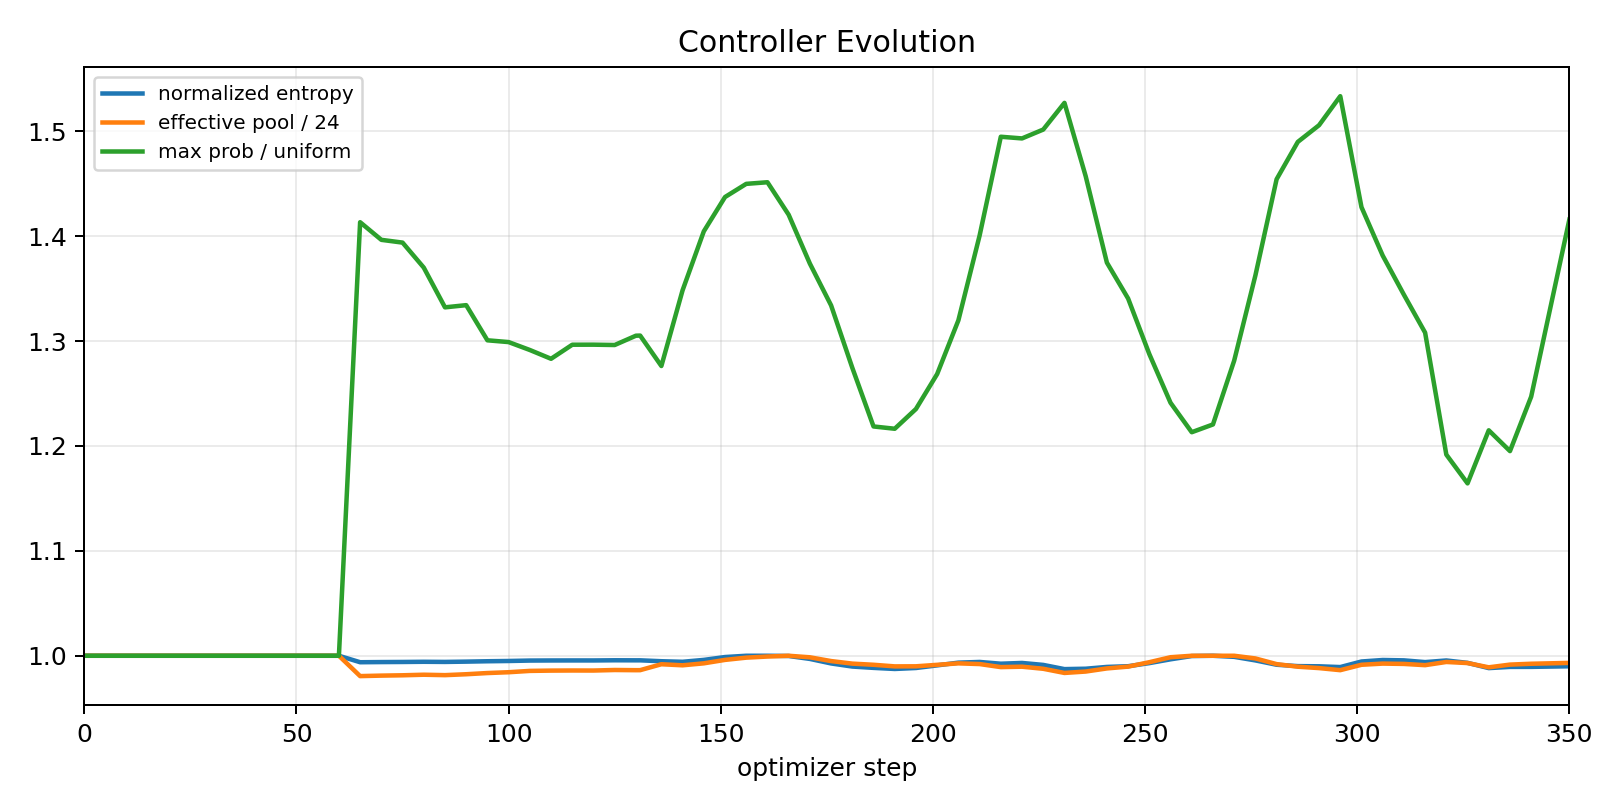
\includegraphics[width=\textwidth]{Figures/controller-evolution-to350.png}
\caption{Controller evolution through optimizer step 350. Entropy is
normalized by $\log 24$; the effective pool is divided by 24; and maximum
probability is divided by the uniform probability $1/24$.}
\label{fig:supp-controller-evolution}
\end{figure*}

\begin{table}[t]
\centering
\small
\begin{tabular}{rrrrr}
\toprule
Step & Groups & $H/\log24$ & Effective pool & Max. prob. \\
\midrule
0 & 0 & 1.000 & 24.00 & 0.0417 \\
151 & 2,366 & 0.999 & 23.91 & 0.0599 \\
201 & 3,166 & 0.991 & 23.79 & 0.0529 \\
251 & 3,966 & 0.993 & 23.85 & 0.0536 \\
301 & 4,766 & 0.995 & 23.79 & 0.0595 \\
350 & 5,550 & 0.990 & 23.84 & 0.0590 \\
\bottomrule
\end{tabular}
\caption{Selected controller snapshots. Probabilities are averaged across
support intents.}
\label{tab:supp-controller-snapshots}
\end{table}

At the final recorded snapshot, every state and all 192 intent--state units
have been observed. The mean state distribution remains broad because boundary
values are intent-conditioned: a state that is informative for one support
intent need not be informative for another. This is consistent with the design
goal of reallocating probability within each intent while preserving global
coverage.

\begin{figure*}[t]
\centering
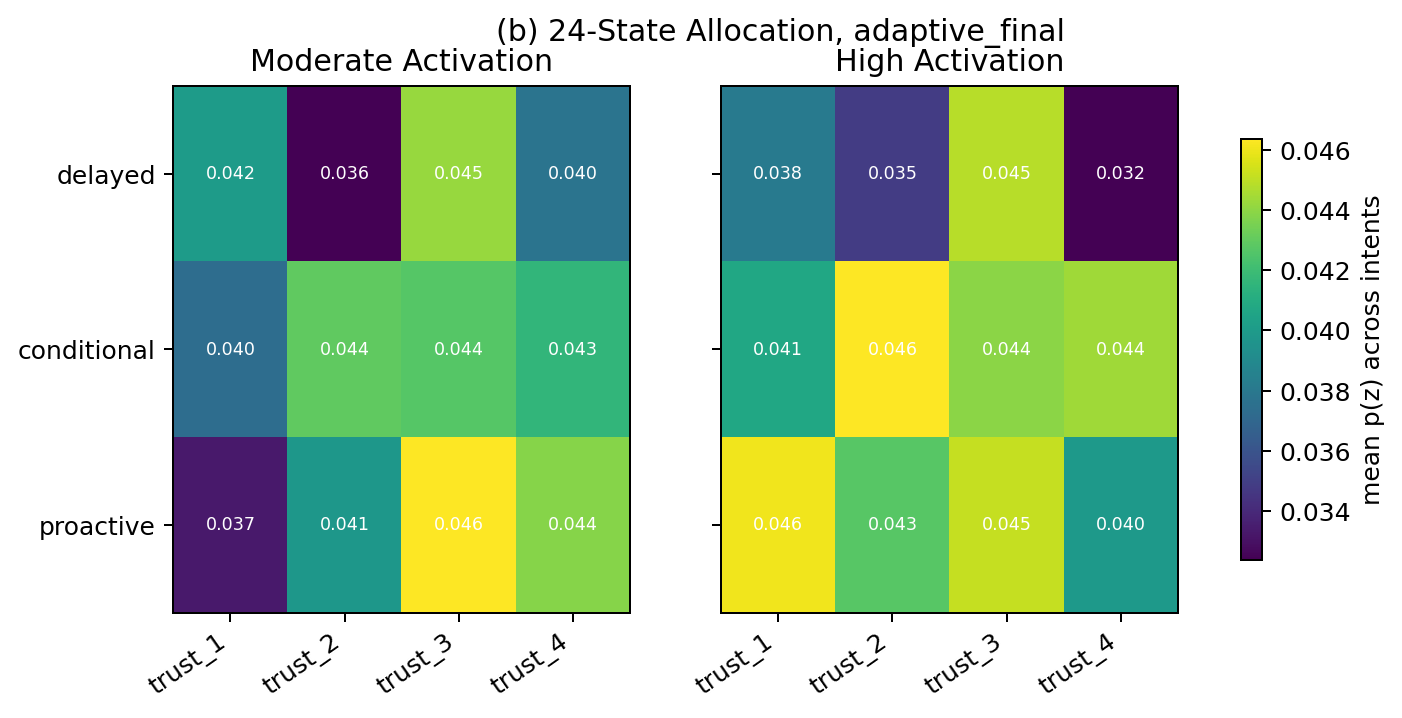
\includegraphics[width=0.82\textwidth]{Figures/controller-state24-heatmaps.png}
\caption{Mean final allocation over the 24 interaction states, averaged across
the eight support intents. Rows are disclosure levels, columns are trust
levels, and the panels separate moderate and high activation.}
\label{fig:supp-state-heatmap}
\end{figure*}

\section{Interaction-State Adherence Audit}
We audit 120 complete multi-turn trajectories, sampling five trajectories from
each of the 24 states. A held-out Qwen3-Max judge sees only the dialogue and not
the requested labels, then predicts each behavioral level and checks semantic
preservation. We separately inspect 30 randomly sampled trajectories manually.

\begin{table}[t]
\centering
\small
\begin{tabular}{lrr}
\toprule
State dimension & Accuracy & Macro-F1 \\
\midrule
Disclosure readiness & 86.7 & 86.7 \\
Emotional activation & 92.5 & 92.5 \\
Relational trust & 82.5 & 82.1 \\
All dimensions correct & 68.3 & -- \\
\bottomrule
\end{tabular}
\caption{Behavioral adherence across all 24 interaction states (\%).}
\label{tab:supp-state-adherence}
\end{table}

\begin{table}[t]
\centering
\small
\begin{tabular}{lr}
\toprule
Semantic constraint & Pass rate \\
\midrule
Persona preserved & 98.3 \\
Event facts preserved & 97.5 \\
Hidden need preserved & 96.7 \\
Support intent preserved & 98.3 \\
No dimension-name leakage & 99.2 \\
No level/difficulty leakage & 98.3 \\
All semantic constraints & 92.5 \\
\bottomrule
\end{tabular}
\caption{Scenario preservation and metadata non-disclosure (\%).}
\label{tab:supp-state-semantics}
\end{table}

The audit supports both requirements of the interaction-state design. First,
requested differences are recoverable from generated behavior, with single-axis
accuracy between 82.5\% and 92.5\%. Second, 92.5\% of trajectories jointly
preserve the persona, event, and hidden need while avoiding metadata leakage.
On the 30-case manual subset, human decisions agree with the automatic audit in
90.0\% of cases, with Cohen's $\kappa=0.89$.

\section{Reproduction Workflow}
The following sequence reproduces the main-method training path contained in
the archive.
\begin{enumerate}
  \item Validate the training manifest with
  \texttt{scripts/validate\_training\_scenarios.py}. The command checks row
  count, unique IDs, required fields, and the eight intent categories.
  \item Supply a local Qwen3-8B path and an output directory through environment
  variables. Supply the simulator credential only through the process
  environment; no key is stored in the archive.
  \item Run the main launcher in \texttt{launch/}. It exports the controller
  settings in Table~\ref{tab:supp-training-config}, starts the distributed
  workers, and writes the SQLite controller database to the configured local
  POSIX path.
  \item For interrupted jobs, resume the model checkpoint and provide the
  preserved controller database through
  \texttt{EGSEC\_CONTROLLER\_STATE\_FILE}.
  \item Run the included unit tests before training. They cover state-prompt
  composition, hierarchical estimates, exploration floors, atomic updates,
  and incomplete-group behavior.
\end{enumerate}

The code-and-data supplement is intentionally scoped to the new method and its
direct verification utilities, consistent with the submitted reproducibility
checklist. Third-party model weights and benchmark implementations remain under
their respective distributions.
